% ============================================================================
%   Comprehensive Research Report on the Universal GUDS-EDL Architecture
%   Mathematical Foundations, Multi-Agent Dynamics, and Clinical Applications
%
%   File: guds_edl_report_en.tex
%   Version: 2.0 (Updated 06/2026)
%   Language: English
% ============================================================================

\documentclass[letterpaper]{article} % DO NOT CHANGE THIS
\usepackage{aaai}  % DO NOT CHANGE THIS
\usepackage{times}  % DO NOT CHANGE THIS
\usepackage{helvet}  % DO NOT CHANGE THIS
\usepackage{courier}  % DO NOT CHANGE THIS
\usepackage[hyphens]{url}  % DO NOT CHANGE THIS
\usepackage{graphicx} % DO NOT CHANGE THIS
\urlstyle{rm} % DO NOT CHANGE THIS
\def\UrlFont{\rm}  % DO NOT CHANGE THIS
\frenchspacing  % DO NOT CHANGE THIS
\setlength{\pdfpagewidth}{8.5in} % DO NOT CHANGE THIS
\setlength{\pdfpageheight}{11in}
\setcounter{secnumdepth}{2}
%%%%%%%%%%
% PDFINFO for PDFLATEX
\pdfinfo{
/Title (GUDS-EDL: Generalized Uncertainty-Guided Dynamic Sparsification for Evidential Long-Tailed Learning)
/Author (Anonymous Authors)
}
%%%%%%%%%%
 % DO NOT CHANGE THIS

% --- Additional Packages ---
\usepackage[utf8]{inputenc}
\usepackage[english]{babel}
\usepackage{amsmath, amssymb, amsthm, bm}
\usepackage{booktabs}
\usepackage{multirow}
\usepackage{array}
\usepackage{adjustbox}
\usepackage{placeins}
\usepackage{stfloats}
\usepackage{float}
\usepackage{algorithm}
\usepackage{algorithmic}
\usepackage{enumitem}
\usepackage{tikz}
\usetikzlibrary{arrows.meta, positioning}
\usepackage[table]{xcolor}
\usepackage{colortbl}
\usepackage[colorlinks=true,linkcolor=black,citecolor=blue,urlcolor=blue]{hyperref}

\newcolumntype{C}{>{\centering\arraybackslash}c}

% --- Custom commands ---
\newcommand{\Dir}{\text{Dir}}
\newcommand{\KL}{\text{KL}}
\newcommand{\R}{\mathbb{R}}
\newcommand{\E}{\mathbb{E}}
\newcommand{\Norm}{\text{Norm}}
\newcommand{\softplus}{\text{Softplus}}
\newcommand{\pospart}[1]{\left[#1\right]_+}
\DeclareMathOperator*{\argmax}{arg\,max}
\DeclareMathOperator{\TopTwo}{Top2}

\hbadness=10000
\vbadness=10000
\hfuzz=10pt
\vfuzz=4pt
\raggedbottom
\setlength{\textfloatsep}{10pt plus 2pt minus 3pt}
\setlength{\dbltextfloatsep}{10pt plus 2pt minus 3pt}
\setlength{\floatsep}{8pt plus 2pt minus 2pt}
\setlength{\dblfloatsep}{8pt plus 2pt minus 2pt}

\newtheorem{remark}{Remark}
\newtheorem{lemma}{Lemma}
\newtheorem{proposition}{Proposition}

% ============================================================================
\title{GUDS-EDL: Generalized Uncertainty-Guided Dynamic Sparsification for Evidential Long-Tailed Learning}
\author{Anonymous Authors}

\begin{document}

\begin{abstract}
Extreme imbalanced classification appears across many real-world domains, including industrial defect detection, fraud detection, autonomous driving edge-case recognition, and safety-critical medical screening. Standard dense neural networks often overfit majority classes and produce overconfident predictions on rare classes, while conventional pruning techniques ignore uncertainty signals. 

We propose \textbf{GUDS-EDL}, a general-purpose uncertainty-guided dynamic sparse evidential learning framework. GUDS-EDL combines Dirichlet evidential learning with strict NVIDIA 2:4 structured sparsity for hardware-compatible sparsity. An uncertainty-guided pruner removes noise-amplifying connections using signed gradients of an evidential risk ratio, while an evidence-seeking regrower restores capacity in representation-deficient regions. A topology cache reduces mask update overhead, and Evidential Focal Loss stabilizes sparse training under severe imbalance. 

We formulate GUDS-EDL as a methodological framework for long-tailed and rare-event evidential learning, and instantiate it on ISIC 2024 as a high-stakes extreme-imbalance case study. We further design a multi-benchmark evaluation protocol covering controlled long-tailed recognition and industrial anomaly detection, which will be used to assess the framework beyond the medical domain.
\end{abstract}

\section{Introduction and Research Background}\label{sec:intro}

The deployment of large-scale deep learning models in real-world systems often faces extreme class imbalance, where rare but high-cost events are vastly underrepresented. This phenomenon, known as the long-tailed distribution, occurs naturally across critical domains including industrial defect detection, financial fraud, autonomous driving edge cases, safety violations, and medical abnormalities. In these high-stakes regimes, models must be simultaneously accurate on rare classes, precisely calibrated to express uncertainty when ignorant, and efficient enough for low-latency deployment.

Standard softmax-based neural networks are notoriously vulnerable to these challenges, tending to overfit majority classes and produce overconfident predictions on out-of-distribution or ambiguous minority samples~\cite{guo2017calibration}. Evidential Deep Learning (EDL)~\cite{sensoy2018evidential} mitigates overconfidence by parameterizing a higher-order Dirichlet distribution, directly representing the model's ignorance (epistemic uncertainty) and data noise (expected categorical entropy)~\cite{malinin2018predictive}. Concurrently, Dynamic Sparse Training (DST)~\cite{evci2020rigging} addresses computational constraints by dynamically exploring sparse network topologies from scratch. However, existing DST methods prune connections based solely on weight magnitudes or task gradients, remaining entirely blind to uncertainty signals.

To bridge this gap, we introduce \textbf{Generalized Uncertainty-Guided Dynamic Sparsification for Evidential Long-Tailed Learning (GUDS-EDL)}, a framework that integrates Evidential Learning with strict NVIDIA 2:4 structured sparsity. The network topology is dynamically optimized by two computational agents: an \textbf{Uncertainty-Guided Pruner} (inspired by biological Microglia) that removes noise-amplifying connections using the signed gradients of an evidential risk ratio, and an \textbf{Evidence-Seeking Regrower} (inspired by Astrocytes) that restores links at nodes plagued by high epistemic uncertainty. Medical screening is used as one representative high-stakes instantiation, but the proposed framework does not rely on medical assumptions and generalizes to broader rare-event tasks.

\paragraph{Main Contributions.} To our knowledge, this is the first framework to leverage Dirichlet uncertainty signals to guide NVIDIA 2:4 structured dynamic sparse training under extreme class imbalance. Specifically, our primary contributions are:
\begin{itemize}
    \item \textbf{EDL Contribution:} An imbalance-aware evidential objective incorporating dampened class weights and an asymmetric KL divergence penalty, enabling robust rare-event sensitivity.
    \item \textbf{DST Contribution:} An uncertainty-guided connection pruning and regrowth mechanism under strict 2:4 structured sparsity constraints, driven by epistemic and categorical entropy gradients.
    \item \textbf{Real-World Case Study:} We formulate a multi-benchmark evaluation protocol for long-tailed recognition and industrial anomaly detection, and currently instantiate the framework on the ISIC 2024 cohort as a high-stakes extreme-imbalance case study for adaptive operating threshold configurations.
\end{itemize}

\section{Related Work}\label{sec:related}

\paragraph{Long-Tailed and Extreme Imbalanced Learning.} Long-tailed recognition has been extensively studied through re-sampling, re-weighting, margin adjustment, classifier decoupling, and contrastive learning. Class-Balanced Loss~\cite{cui2019class} reweights examples according to the effective number of samples, while LDAM-DRW~\cite{cao2019learning} introduces label-distribution-aware margins with deferred re-weighting to improve tail-class decision boundaries. Logit Adjustment~\cite{menon2021long} and Balanced Softmax~\cite{ren2020balanced} reinterpret long-tailed learning as a label-prior shift problem and modify logits or softmax normalization accordingly. Other works decouple representation learning from classifier balancing~\cite{kang2019decoupling}, showing that strong representations can be learned under natural sampling and later adapted with a balanced classifier. Architectures such as BBN~\cite{zhou2020bbn} and contrastive objectives such as PaCo~\cite{cui2021parametric} further improve head-tail trade-offs. Unlike these methods, GUDS-EDL does not only rebalance the classification loss; it uses evidential uncertainty signals to adapt the sparse topology itself, targeting representation-deficient regions under extreme imbalance.

\paragraph{Evidential and Dirichlet-Based Uncertainty Estimation.} Evidential Deep Learning (EDL)~\cite{sensoy2018evidential} replaces point-estimate softmax confidence with a Dirichlet distribution over class probabilities, enabling single-forward-pass uncertainty estimation. Related Dirichlet-prior methods, such as Prior Networks~\cite{malinin2018predictive} and Posterior Networks~\cite{charpentier2020posterior}, further model predictive distributions for OOD detection and calibration under dataset shift. Recent EDL variants improve the reliability of evidence learning: Fisher Information-based EDL~\cite{deng2023fisher} reweights evidential objectives using sample informativeness, R-EDL~\cite{chen2023redl} relaxes nonessential subjective-logic assumptions, and Flexible EDL~\cite{yoon2025flexible} replaces the fixed Dirichlet assumption with a more expressive flexible Dirichlet family. Recent advances further extend these concepts: ANEDL~\cite{yu2024anedl} explores open-set semi-supervised evidential learning, while Evidence Contraction~\cite{wu2024evidence} analyzes activation constraints in deep evidential regression. However, recent critiques~\cite{shen2024mirage} argue that EDL uncertainties should not be interpreted as exact Bayesian epistemic uncertainty. Following this view, GUDS-EDL uses Dirichlet vacuity and expected categorical entropy as practical structural adaptation signals rather than as calibrated Bayesian uncertainty bounds.

\paragraph{Calibration, Selective Prediction, and Failure Detection.} Reliable deployment under rare-event imbalance requires not only high minority recall but also calibrated confidence and the ability to abstain. \citeauthor{guo2017calibration}~(\citeyear{guo2017calibration}) showed that modern neural networks are often miscalibrated and that temperature scaling is a strong post-hoc baseline. Selective classification~\cite{geifman2017selective,geifman2019selectivenet} formalizes abstention through the risk-coverage trade-off, allowing a model to reject uncertain samples in mission-critical applications. AURC~\cite{ding2020revisiting} is widely used to summarize selective prediction performance, although recent studies caution that aggregate risk-coverage metrics can hide important working-point behavior~\cite{jaeger2023call,traub2024overcoming}. Accordingly, GUDS-EDL reports both calibration metrics and operating-point metrics such as high-recall specificity and quality-gated coverage-risk behavior.

\paragraph{Dynamic Sparse Training and Structured Sparsity.} Classical pruning pipelines~\cite{han2016deep,frankle2019lottery} compress dense networks after training, whereas dynamic sparse training maintains sparse connectivity throughout optimization. SET~\cite{mocanu2018scalable} evolves a sparse topology during training, SNFS~\cite{dettmers2019sparse} uses sparse momentum to grow useful connections, and RigL~\cite{evci2020rigging} updates sparse topology through magnitude-based pruning and gradient-based regrowth under a fixed parameter budget. Recent advances include PFFDST~\cite{li2025pffdst}, which explores parameter-freezing-based federated dynamic sparse training. However, most centralized DST methods focus on unstructured sparsity, which is difficult to accelerate on modern hardware. Structured DST methods such as SRigL~\cite{lasby2023srigl} move toward hardware-compatible sparsity patterns, while NVIDIA Sparse Tensor Cores motivate strict 2:4 sparsity for efficient deployment~\cite{mishra2021accelerating}. GUDS-EDL differs from these methods by making topology evolution uncertainty-aware: connections are pruned and regrown according to evidential risk, vacuity, and class-conditioned rare-event utility rather than weight magnitude or task gradient alone.

\paragraph{Rare-Event Benchmarks and High-Stakes Case Studies.} Long-tailed recognition is commonly evaluated on controlled CIFAR-LT variants and large-scale benchmarks such as iNaturalist~\cite{liu2019large}. Industrial anomaly detection benchmarks such as MVTec AD~\cite{bergmann2019mvtec} provide real-world rare-event inspection settings, while ISIC 2024 provides a high-stakes medical rare-event case study based on 3D total body photography lesion crops. In the current work, we report an initial ISIC 2024 case study and define CIFAR-100-LT and MVTec AD as planned benchmarks for future validation. This distinction avoids conflating framework generality with completed multi-domain empirical evidence.

\section{Mathematical Foundations: Subjective Logic and Dirichlet Distribution}\label{sec:math}

We replace the traditional softmax activation with mathematical foundations from Subjective Logic (SL)~\cite{josang2016subjective}, mapping network outputs to the parameters of a Dirichlet distribution conjugate prior~\cite{sensoy2018evidential}.

\subsection{Dirichlet Distribution Parameterization}
For a $K$-class problem, we parameterize the non-negative evidence vector $\bm{e} \ge \bm{0}$ from logits $\bm{z} \in \R^K$ using the Softplus activation:
\begin{equation}\label{eq:softplus}
    e_c = \ln(1 + \exp(z_c)), \quad c = 1, \ldots, K
\end{equation}
\begin{remark}[Why not use ReLU?]
ReLU truncates negative logits to zero, resulting in zero gradients for those activations and permanently trapping evidence at $e_c = 0$, which freezes the Dirichlet state on the zero-evidence simplex.
\end{remark}
The probability density function (PDF) of the Dirichlet distribution for a probability vector $\bm{p} = [p_1, \dots, p_K]^T$ on the $K$-dimensional simplex $\Delta^K$ is defined as:
\begin{equation}\label{eq:dirichlet_pdf}
    \Dir(\bm{p} \mid \bm{\alpha}) = \frac{1}{B(\bm{\alpha})} \prod_{c=1}^K p_c^{\alpha_c - 1} = \frac{\Gamma(S)}{\prod_{c=1}^K \Gamma(\alpha_c)} \prod_{c=1}^K p_c^{\alpha_c - 1}
\end{equation}
where $\Gamma(\cdot)$ is the Gamma function, and $B(\bm{\alpha})$ is the multivariate Beta function. The Dirichlet concentration parameters $\bm{\alpha}$ are defined by adding a uniform prior to the evidence:
\begin{equation}\label{eq:alpha}
    \alpha_c = e_c + 1.0
\end{equation}
where $S = \sum_{c=1}^K \alpha_c$ is the Dirichlet strength (total evidence). In Subjective Logic (SL), a multinomial opinion maps this evidence to belief masses $b_c \ge 0$ and a vacant belief mass (uncertainty) $u_e \ge 0$. The belief mass for class $c$ is defined as:
\begin{equation}\label{eq:belief}
    b_c = \frac{e_c}{S}
\end{equation}
The core identity of Subjective Logic guarantees that the sum of belief masses and epistemic uncertainty equals unity:
\begin{equation}\label{eq:sl_identity}
    \sum_{c=1}^K b_c + u_e = 1
\end{equation}
which establishes the strict mathematical coupling between the evidence vector $\bm{e}$, class belief representations, and the vacant belief mass. Under this formulation, the expected probability for class $c$ is:
\begin{equation}\label{eq:p_hat}
    \hat{p}_c = \E[p_c] = \frac{\alpha_c}{S}
\end{equation}
The effects of extreme class imbalance are strictly handled via Evidential Focal Loss (which modulates loss gradients based on class frequencies) rather than by altering the Dirichlet prior. This ensures that the total evidence $S$ remains well-bounded ($S \ge K$), preserving the mathematical consistency of the epistemic uncertainty limits.

\subsection{Decomposition of Predictive Uncertainty}\label{subsec:uncertainties}
Under Subjective Logic, predictive uncertainty can be decomposed into complementary components that capture different aspects of the predicted distribution. Following recent critiques of Evidential Deep Learning \cite{shen2024mirage}, we explicitly state that we do not claim true Bayesian epistemic uncertainty. Instead, we define mathematically well-formed uncertainty proxies that are used as structural adaptation signals.

\paragraph{Dirichlet Vacuity / Evidence-Based Uncertainty ($u_e$):} Models the network's lack of knowledge (e.g., on OOD or rare data). Defined as the vacant belief mass in Subjective Logic:
\begin{equation}\label{eq:u_e}
    u_e = \frac{K}{S} = \frac{K}{\sum_{c=1}^K \alpha_c}
\end{equation}
For finite logits under Eq.~\ref{eq:softplus}, $u_e \in (0, 1)$, with supremum $1$ approached in the zero-evidence limit. We utilize this vacuity metric as a structural adaptation signal rather than a strict epistemic uncertainty bound.

\paragraph{Entropy-Based Ambiguity Proxy ($u_a$):} Used as a data-ambiguity/noise proxy (similar to aleatoric uncertainty), this measures the expected Shannon entropy of the multinomial distribution under the Dirichlet conjugate prior \cite{malinin2018predictive}:
\begin{equation}\label{eq:u_a}
    u_a = \sum_{c=1}^K \frac{\alpha_c}{S} \left[\psi(S + 1) - \psi(\alpha_c + 1)\right]
\end{equation}
where $\psi(x)$ is the digamma function. For any $K > 1$, $u_a \ge 0$ due to the strict monotonicity of the digamma function. In practical implementations, to protect against floating-point inaccuracies, $u_a \leftarrow \max(u_a, 0.0)$ is applied.

\begin{proposition}[Validity of Evidential State]
\label{prop:evidential_validity}
For any logits $\bm{z}\in\R^K$ under the Softplus evidence map in Eq.~\ref{eq:softplus}, the induced Dirichlet parameters satisfy $\alpha_c>1$, $S>K$, $\hat{\bm{p}}\in\Delta^K$, $u_e\in(0,1)$ for finite logits with supremum $1$ as all evidence tends to zero, and $u_a\ge0$.
\end{proposition}

\paragraph{Theoretical Scope.}
The quantities $u_e$ and $u_a$ are therefore valid bounded/non-negative signals derived from a proper Dirichlet distribution. We use them to drive topology adaptation and selective prediction; we do not require or assert that they are exact Bayesian posterior epistemic and aleatoric uncertainties. Full proofs of all propositions are provided in Appendix~\ref{app:proofs}.


\section{Universal GUDS-EDL Framework}\label{sec:methodology}

\textbf{Transparency Disclaimer on Terminology}: We draw metaphorical inspiration from biological glial cells (Microglia and Astrocytes) to guide our Dynamic Sparse Training. To maintain clarity for general computer vision and anomaly detection literature, we refer to these computational mechanisms formally as the \textbf{Uncertainty-Guided Pruner} and the \textbf{Evidence-Seeking Regrower}, using the biological terms solely as mnemonic aliases for backward compatibility.


\begin{figure}[t]
\centering
\resizebox{\columnwidth}{!}{%
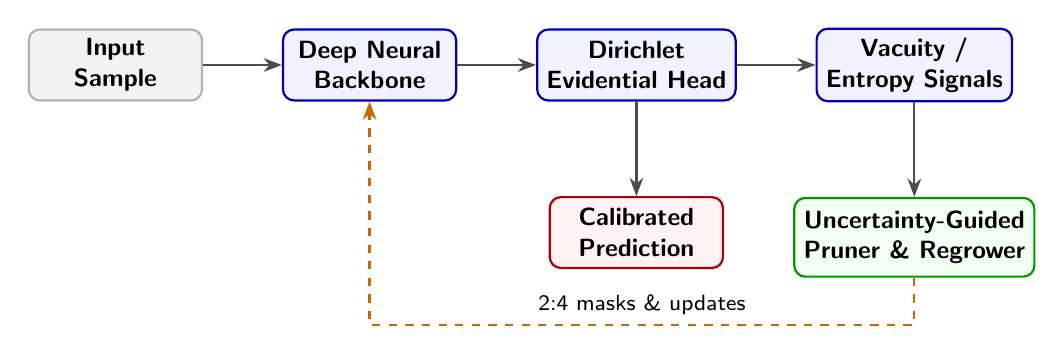
\begin{tikzpicture}[
    node distance=1.2cm and 1.0cm,
    box/.style={
        draw=blue!70!black,
        fill=blue!5,
        rounded corners,
        align=center,
        minimum width=2.2cm,
        minimum height=0.9cm,
        font=\small\sffamily\bfseries,
        thick
    },
    agent/.style={
        draw=green!60!black,
        fill=green!5,
        rounded corners,
        align=center,
        minimum width=2.4cm,
        minimum height=1.0cm,
        font=\small\sffamily\bfseries,
        thick
    },
    pred/.style={
        draw=red!70!black,
        fill=red!5,
        rounded corners,
        align=center,
        minimum width=2.2cm,
        minimum height=0.9cm,
        font=\small\sffamily\bfseries,
        thick
    },
    arrow/.style={
        ->,
        >=Stealth,
        thick,
        draw=black!70
    },
    feedback/.style={
        ->,
        >=Stealth,
        thick,
        dashed,
        draw=orange!80!black
    }
]

% Nodes
\node (img) [box, fill=gray!10, draw=gray!60] {Input\\Sample};
\node (backbone) [box, right=of img] {Deep Neural\\Backbone};
\node (head) [box, right=of backbone] {Dirichlet\\Evidential Head};
\node (signals) [box, right=of head] {Vacuity /\\Entropy Signals};
\node (agents) [agent, below=of signals] {Uncertainty-Guided\\Pruner \& Regrower};
\node (pred) [pred, below=of head] {Calibrated\\Prediction};

% Paths
\draw [arrow] (img) -- (backbone);
\draw [arrow] (backbone) -- (head);
\draw [arrow] (head) -- (signals);
\draw [arrow] (head) -- (pred);
\draw [arrow] (signals) -- (agents);
\draw [feedback] (agents.south) -- ++(0,-0.6) -| node[above, pos=0.25, font=\footnotesize\sffamily] {2:4 masks \& updates} (backbone.south);

\end{tikzpicture}%
}
\caption{Overview of the Universal GUDS-EDL architecture. Evidential uncertainty is used both for calibrated prediction and for dynamic sparse topology adaptation.}
\label{fig:overview}
\end{figure}

\subsection{Two-Tier Dynamic Sparsity under NVIDIA 2:4 Constraint}
Following the backbone-agnostic formulation of Evidential Deep Learning \cite{sensoy2018evidential}, we apply GUDS-EDL to a general feature extractor $f_\theta(\cdot)$ by wrapping the convolutional kernels and linear projection matrices that dominate the parameter count. We decouple representational weight learning from network morphology updates by defining two tiers of variables:
\begin{itemize}
    \item \textbf{Prediction Tier:} Contains the active weights $\bm{W}^{(l)}$ optimized via AdamW to minimize the task loss.
    \item \textbf{Morphological Tier:} Contains continuous latent scores $\bm{V}^{(l)}$ representing connection vitality, initialized to $|W_{ij}^{(0)}|$ to avoid pruning shock. The binary mask $\bm{M}^{(l)}$ is derived from $\bm{V}^{(l)}$.
\end{itemize}
We enforce the hardware-supported NVIDIA 2:4 structured sparsity constraint, which requires exactly 2 non-zero elements in every contiguous block of 4 weights along the inner dimension. To ensure broad architectural compatibility, we define a structural reshape operator before applying the mask. For 2D convolutional layers with kernel size $K_h \times K_w$, the tensor $\bm{W}^{(l)} \in \R^{C_{\text{out}} \times C_{\text{in}} \times K_h \times K_w}$ is reshaped to $\bm{W}_{\text{flat}}^{(l)} \in \R^{C_{\text{out}} \times (C_{\text{in}}K_hK_w)}$; zero-padding is applied only when the inner dimension is not divisible by 4 and is removed after masking. For transformer or MLP projections, $\bm{W}^{(l)} \in \R^{D_{\text{out}} \times D_{\text{in}}}$ already has this flattened form. For row $i$ and 4-block $k$, the mask is:
\begin{equation}\label{eq:mask}
    \begin{aligned}
    I_{i,k}^{(l)} &= \TopTwo_{j \in \{0,1,2,3\}}
    V_{\text{flat}, i, 4k+j}^{(l)},\\
    M_{\text{flat}, i, 4k+j}^{(l)} &=
    \begin{cases}
        1 & \text{if } j \in I_{i,k}^{(l)},\\
        0 & \text{otherwise.}
    \end{cases}
    \end{aligned}
\end{equation}
The mask is then reshaped back to the original tensor dimensions. The effective weights used in the forward pass are $\bm{W}_{\text{eff}} = \bm{W} \odot \bm{M}$.

\begin{proposition}[2:4 Feasibility Preservation]
\label{prop:24_feasibility}
Assume each wrapped weight tensor is flattened along its inner dimension and padded, if necessary, so that every row decomposes into disjoint contiguous 4-blocks. The mask generated by Eq.~\ref{eq:mask} satisfies exact NVIDIA 2:4 sparsity in every block after every mask refresh, and the resulting active density in each wrapped layer is exactly $50\%$ over the padded representation.
\end{proposition}

\subsection{Decoupled Morphological Updates, Ghost Gradients, and Mask Caching}
To prevent "optimizer hijacking" where AdamW weight decay and parameter momentum interfere with the continuous latent topology, we decouple structural vitality updates from the standard prediction optimizer. Since $\bm{W}_{\text{eff}}=\bm{W}\odot\bm{M}$, backpropagation gives $\nabla_{\bm{W}}\bm{W}_{\text{eff}}=\bm{M}$, so prediction gradients and weight decay only act on active links. Dormant links therefore need a separate structural memory rather than instantaneous masked gradients.

\begin{proposition}[Masked-Gradient Isolation]
\label{prop:masked_gradient}
Let $L$ be any differentiable mini-batch training loss evaluated through $\bm{W}_{\text{eff}}=\bm{W}\odot\bm{M}$ with a fixed binary mask $\bm{M}$ during the mini-batch. Then
\begin{equation}\label{eq:masked_gradient}
    \nabla_{\bm{W}} L
    =
    \nabla_{\bm{W}_{\text{eff}}} L \odot \bm{M}.
\end{equation}
Consequently, inactive entries with $M_{ij}=0$ receive zero instantaneous task gradient and cannot be regrown by ordinary masked backpropagation alone.
\end{proposition}

Let $\bar{G}_{ij}^{(t)}$ denote an exponential moving average of historical growth evidence for connection $(i,j)$ at structural update $t$. We update this memory using only links that are active during the proxy structural pass:
\begin{equation}\label{eq:ghost_gradient}
    \bar{G}_{ij}^{(t)}
    = \beta_g \bar{G}_{ij}^{(t-1)}
    + (1-\beta_g)\,\mathbb{I}[M_{ij}^{(t)}=1]\,G_{ij}^{(t)} .
\end{equation}
This keeps the physical parameter storage dense, but avoids materializing a dense auxiliary backpropagation graph for every dormant parameter at every mini-batch. The structural scores $V_{ij}$ are updated once per epoch from an amortized proxy batch, which reduces high-frequency topology noise while preserving a route for regrowth of recently pruned links.

To eliminate redundant sorting and top-k operations over tens of millions of parameters during standard iterations, we introduce a Morphological Cache. The computed mask $\bm{M}$ is registered as a non-persistent buffer and kept static for the remainder of the epoch. This epoch-level caching serves as a structural regularizer and avoids the extreme slowdown associated with running auxiliary structural backpropagation at every mini-batch step.

\subsection{Pruning and Regrowth Complementary Topology Heuristics}
Topology evolution is driven by complementary heuristics. Within the GUDS-EDL framework, we adopt a simplified computational abstraction where the Uncertainty-Guided Pruner and Evidence-Seeking Regrower are assigned distinct, orthogonal roles (pruning and growing, respectively) to enable decoupled control over network connection density and explore the topological search space efficiently.

\paragraph{Uncertainty-Guided Pruning.}
To avoid relying on entropy gradients that can saturate as the Dirichlet strength $S$ grows large, we define the evidential risk ratio $R = \frac{u_a}{u_e + \epsilon}$. With the current mask held fixed during the proxy structural pass, both $u_a$ and $u_e$ depend on $\bm{\alpha}$, $S$, logits $\bm{z}$, and ultimately $\bm{W}$, so the pruning gradient is computed by the chain rule:
\begin{equation}\label{eq:r_chain_main}
    \frac{\partial R}{\partial w_{ij}}
    =
    \frac{1}{u_e+\epsilon}\frac{\partial u_a}{\partial w_{ij}}
    -\frac{u_a}{(u_e+\epsilon)^2}
    \frac{\partial u_e}{\partial w_{ij}} .
\end{equation}
A full expansion through the Dirichlet parameters is given in Appendix~\ref{app:r_chain}. To construct a directional harmfulness criterion rather than a mere sensitivity heuristic, we evaluate the first-order Taylor expansion of the risk after removing a connection ($w_{ij} \to 0$): $\Delta R \approx -w_{ij}\frac{\partial R}{\partial w_{ij}}$. Therefore, positive $w_{ij}\frac{\partial R}{\partial w_{ij}}$ indicates that removal is expected to reduce $R$. The pruning force is the Signed First-Order Removal Effect:
\begin{equation}\label{eq:C_ij}
    C_{ij}
    =
    \operatorname{Rank}\left(
    \pospart{w_{ij}\frac{\partial R}{\partial w_{ij}}}
    \right),
    \qquad
    \pospart{x}=\max(x,0).
\end{equation}
By applying the positive-part operator, we ignore highly sensitive connections whose removal would increase uncertainty (i.e., highly useful features). This ensures the pruner explicitly targets and prunes noise-amplifying, overconfident connections rather than blindly pruning high-magnitude gradients.

\begin{proposition}[Signed First-Order Pruning Criterion]
\label{prop:signed_pruning}
Let $R$ be differentiable with respect to $w_{ij}$ in a neighborhood of the current weight. If $w_{ij}\frac{\partial R}{\partial w_{ij}}>0$, then setting $w_{ij}$ to zero decreases $R$ to first order. If $w_{ij}\frac{\partial R}{\partial w_{ij}}<0$, removing the connection increases $R$ to first order.
\end{proposition}

\paragraph{Evidence-Seeking Regrowth.}
A naive maximization of the Kullback-Leibler Divergence from a Uniform Prior ($\Dir(\mathbf{1})$) risks indiscriminately inflating evidence for majority classes, leading to "junk evidence accumulation." To bias structural recovery toward representation-deficient rare-event samples without changing the Dirichlet prior, we formulate a sample-level Class-Conditioned Uncertainty-Gated growth objective. We gate the KL divergence by the sample's ground-truth class weight $\omega_y$ and its current Dirichlet vacuity $u_e$:
\begin{equation}\label{eq:grow_objective}
\begin{split}
    L_{\text{grow}} ={}& \omega_y \cdot u_e \cdot \KL(\Dir(\bm{\alpha}) \parallel \Dir(\mathbf{1})) \\
    ={}& \omega_y \cdot u_e \cdot \Bigg( \ln \Gamma(S) - \sum_{c=1}^K \ln \Gamma(\alpha_c) - \ln \Gamma(K) \\
    &+ \sum_{c=1}^K (\alpha_c - 1)\left[ \psi(\alpha_c) - \psi(S) \right] \Bigg)
\end{split}
\end{equation}
Writing $\mathcal{K}(\bm{\alpha})=\KL(\Dir(\bm{\alpha})\parallel\Dir(\mathbf{1}))$, the corresponding structural gradient factorizes as
\begin{equation}\label{eq:grow_chain}
    \frac{\partial L_{\text{grow}}}{\partial w_{ij}}
    =
    \omega_y
    \left[
    \mathcal{K}(\bm{\alpha})
    \frac{\partial u_e}{\partial w_{ij}}
    +u_e
    \frac{\partial \mathcal{K}(\bm{\alpha})}{\partial w_{ij}}
    \right].
\end{equation}
Thus, $\omega_y$ amplifies the structural saliency of rare-class samples; it does not by itself impose a coordinate-wise preference for increasing $\alpha_y$ over every $\alpha_{c\ne y}$. The direction of recovered connectivity remains determined by the backpropagated evidential gradient through that sample's feature pathway. The corresponding growth score for structural recovery is:
\begin{equation}\label{eq:G_ij}
    G_{ij} = \operatorname{Rank}\left( \left| \frac{\partial L_{\text{grow}}}{\partial w_{ij}} \right| \right)
\end{equation}

\begin{proposition}[Local Regrowth Saliency]
\label{prop:regrowth_saliency}
Let $Q(\bm{W})=L_{\text{grow}}(\bm{W})$ be differentiable at the current weights. Among candidate scalar perturbations $|\delta_{ij}|\le\eta$ applied independently to a connection, the largest possible first-order change in $Q$ is $\eta\left|\frac{\partial Q}{\partial w_{ij}}\right|$. Therefore, ranking dormant or weak connections by $\left|\frac{\partial L_{\text{grow}}}{\partial w_{ij}}\right|$ selects those with the greatest local capacity to alter the class-conditioned evidence-seeking objective.
\end{proposition}

\begin{remark}[Regrowth Is a Saliency Rule]
Proposition~\ref{prop:regrowth_saliency} justifies the regrowth score as a first-order local saliency criterion. It does not claim global optimality of the sparse topology; the final sign and magnitude of active weights are learned by the prediction optimizer after the link becomes active.
\end{remark}

\paragraph{Dormant Regrowth and Anti-Crystallization.}
Since inactive weights receive zero instantaneous task gradients under masking, dormant-link regrowth uses the cached EMA signal in Eq.~\ref{eq:ghost_gradient}. If an entire layer becomes structurally frozen, GUDS-EDL injects layer-normalized exploration noise:
\begin{equation}\label{eq:anti_crystal}
    \tilde{G}_{ij}^{(l)}
    = G_{ij}^{(l)}
    + \mathbb{I}\!\left[
    \max_{ij}G_{ij}^{(l)}
    < \kappa\,\operatorname{EMA}\!\left(\max_{ij}G_{ij}^{(l)}\right)
    \right]\xi_{ij}\,\sigma(\bm{V}^{(l)}),
    \quad \xi_{ij}\sim\mathcal{N}(0,1).
\end{equation}
The latent vitality update combines active-link growth, pruning pressure, and dormant-link memory:
\begin{equation}\label{eq:latent_update}
\begin{aligned}
    \Delta V_{ij}^{(t)}
    &= \mathbb{I}[M_{ij}^{(t)}=1]\left(\tilde{G}_{ij}^{(t)}-C_{ij}^{(t)}\right)
    + \mathbb{I}[M_{ij}^{(t)}=0]\,\rho\,\bar{G}_{ij}^{(t-1)},\\
    \mu_{ij}^{(t)}
    &= \beta_m \mu_{ij}^{(t-1)} + (1-\beta_m)\Delta V_{ij}^{(t)},\\
    V_{ij}^{(t)}
    &\leftarrow
    \operatorname{clamp}\!\left(
    V_{ij}^{(t-1)}+\eta_{\text{struct}}\mu_{ij}^{(t)}
    - \operatorname{mean}(\bm{V}^{(t)}),
    -V_{\max}, V_{\max}
    \right).
\end{aligned}
\end{equation}
After Eq.~\ref{eq:latent_update}, the epoch mask is recomputed by Eq.~\ref{eq:mask}. In our implementation, $\beta_m=0.95$, $\eta_{\text{struct}}=0.02$, and $V_{\max}=5.0$.

\begin{proposition}[Bounded Morphological State]
\label{prop:bounded_scores}
For every structural update using Eq.~\ref{eq:latent_update}, all latent scores satisfy $V_{ij}^{(t)}\in[-V_{\max},V_{\max}]$. Therefore, the structural state remains bounded, and every subsequent mask refresh remains feasible under Proposition~\ref{prop:24_feasibility}.
\end{proposition}

\begin{lemma}[Conditional Top-2 Mask Stability]
\label{lem:mask_stability}
For row $i$ and 4-block $k$, let $V_{(2),i,k}^{(t)}$ and $V_{(3),i,k}^{(t)}$ denote the second- and third-largest vitality scores at structural step $t$, and define the local margin
\begin{equation}\label{eq:top2_margin}
    \gamma_{i,k}^{(t)}
    =
    V_{(2),i,k}^{(t)}-V_{(3),i,k}^{(t)} .
\end{equation}
If each score in the block changes by at most $B_t$, i.e.,
$\|\bm{V}_{i,k}^{(t+1)}-\bm{V}_{i,k}^{(t)}\|_\infty\le B_t$, then the Top-2 mask for that block is unchanged whenever $\gamma_{i,k}^{(t)}>2B_t$.
\end{lemma}

This lemma is a local stability condition, not a convergence guarantee: mask changes can still occur in low-margin blocks. To quantify topology variation empirically, we track
\begin{equation}\label{eq:flip_rate}
    \operatorname{FlipRate}^{(t)}
    =
    \frac{\|\bm{M}^{(t)}-\bm{M}^{(t-1)}\|_0}
    {\|\bm{M}^{(t-1)}\|_0}.
\end{equation}
Structural momentum and epoch-level caching reduce high-frequency score changes, but a decreasing FlipRate curve should be treated as empirical stability evidence rather than proof of global topology convergence.

\paragraph{Summary of Theoretical Guarantees.}
The propositions above establish the properties required for a well-defined uncertainty-guided sparse learning algorithm: valid Dirichlet uncertainty signals (Proposition~\ref{prop:evidential_validity}), exact 2:4 feasibility (Proposition~\ref{prop:24_feasibility}), isolation of prediction gradients from dormant links (Proposition~\ref{prop:masked_gradient}), a differentiable signed first-order pruning rule (Proposition~\ref{prop:signed_pruning} and Eq.~\ref{eq:r_chain_main}), bounded morphology updates (Proposition~\ref{prop:bounded_scores}), and conditional local mask stability (Lemma~\ref{lem:mask_stability}). The regrowth mechanism is justified as a sample-weighted local saliency rule (Proposition~\ref{prop:regrowth_saliency} and Eq.~\ref{eq:grow_chain}) rather than as a global sparse-architecture optimum or a coordinate-wise guarantee on true-class evidence.

\begin{remark}[Role of Residual Connections]
When applied to architectures with residual skip connections, the identity mapping pathways act as safe bypass routes. By preserving identity mapping pathways, they protect spatial information flow from abrupt topological disruption when the network applies 50\% parameter structured sparsity.
\end{remark}

\section{Optimization Framework}\label{sec:optimization}

To address extreme class imbalance, we seamlessly integrate the Evidential Focal Loss (EFL) originally proposed by \citeauthor{zhou2023domain}~(\citeyear{zhou2023domain}). We acknowledge that the core architecture of combining evidential Dirichlet distributions with focal modulation is their direct contribution. Our technical adaptation of their EFL involves incorporating square-root frequency dampening and a novel True-Class Amplified Asymmetric KL Penalty to coordinate with GUDS-EDL's active structured sparsity updates.

Under extreme long-tail distributions, standard symmetric KL regularization penalizes minority classes disproportionately, forcing the model to confidently output the majority class even on ground-truth minority samples. This calibration paradox artificially inflates the Minority Expected Calibration Error (Minority-ECE). To resolve this, we introduce a bounded True-Class Amplification multiplier $\Lambda_{\text{asym}}^{(n)}$ that leverages the weight of the ground-truth class to aggressively suppress false evidence without allowing rare-class gradients to dominate training:
\begin{equation}\label{eq:efl}
\begin{aligned}
    L_{\text{EFL}}(\bm{e}, \bm{y}, t) ={}& \frac{1}{N} \sum_{n=1}^N
    \omega_n \mathcal{F}_n(t) \\
    &\cdot \left[ L_{\text{CE}}^{(n)} + \lambda_{\text{KL}} \mu(t)
    \Lambda_{\text{asym}}^{(n)} L_{\text{KL}}^{(n)} \right]
\end{aligned}
\end{equation}
The dampened per-sample class weight is
\begin{equation}\label{eq:sample_weight}
    \omega_n=\sum_{c=1}^{K}y_c^{(n)}\omega_c,
    \qquad
    \omega_c=\sqrt{\frac{N_{\text{majority}}}{N_c}},
\end{equation}
which prevents the loss scale from exploding under extreme imbalance. The expected cross-entropy under the Dirichlet predictive distribution is:
\begin{equation}\label{eq:dirichlet_ce}
    L_{\text{CE}}^{(n)}
    = \sum_{c=1}^K y_c^{(n)}
    \left[\psi(S^{(n)})-\psi(\alpha_c^{(n)})\right].
\end{equation}
The focal term is applied with stop-gradient confidence so that focal weighting changes sample emphasis without directly distorting the Dirichlet evidence:
\begin{equation}\label{eq:focal_schedule}
\begin{aligned}
    \mathcal{F}_n(t)
    &= \left(1-\operatorname{sg}\!\left[\hat{p}_{y_n}^{(n)}\right]\right)^{\gamma(t)},\\
    \gamma(t)
    &= \gamma_{\max}\frac{1}{2}\left(1-\cos\left(\pi
    \frac{\max(0,t-T_w)}{T-T_w}\right)\right),
    \qquad \gamma_{\max}=1.2 .
\end{aligned}
\end{equation}
For KL regularization, we remove the true-class evidence from the penalty by defining
$\tilde{\alpha}_c^{(n)}=y_c^{(n)}+(1-y_c^{(n)})\alpha_c^{(n)}$. The adjusted KL term is:
\begin{equation}\label{eq:kl_loss_main}
\begin{aligned}
    L_{\text{KL}}^{(n)}
    ={}& \ln \left(
    \frac{\Gamma\left(\sum_{c=1}^K\tilde{\alpha}_c^{(n)}\right)}
    {\Gamma(K)\prod_{c=1}^K\Gamma(\tilde{\alpha}_c^{(n)})}
    \right)\\
    &+\sum_{c=1}^K(\tilde{\alpha}_c^{(n)}-1)
    \left[
    \psi(\tilde{\alpha}_c^{(n)})
    -\psi\!\left(\sum_{c=1}^K\tilde{\alpha}_c^{(n)}\right)
    \right].
\end{aligned}
\end{equation}
The annealing coefficient is $\mu(t)=\min(1.0,t/t_{\text{anneal}})$ with $t_{\text{anneal}}=10$, and the bounded asymmetric multiplier is
\begin{equation}\label{eq:asym_multiplier}
    \Lambda_{\text{asym}}^{(n)}
    = \min(\omega_{y_n},\Lambda_{\max}),
    \qquad \Lambda_{\max}=10.0 .
\end{equation}
The overall training objective is simply
\begin{equation}\label{eq:total_loss}
    L_{\text{total}}=L_{\text{EFL}}(\bm{e},\bm{y},t).
\end{equation}

\begin{proposition}[Controlled Imbalance Modulation]
\label{prop:controlled_modulation}
For each sample $n$, the stop-gradient focal factor $\mathcal{F}_n(t)$ makes the EFL gradient a non-negative sample reweighting of the Dirichlet CE/KL gradients with respect to the evidence parameters, rather than introducing an additional derivative path through $\hat{p}_{y_n}^{(n)}$. The asymmetric KL component is explicitly bounded by $\Lambda_{\max}$.
\end{proposition}

\paragraph{Learning Rate and Loss-Scale Warmup.}
During the first epoch, the learning rate is linearly warmed from $\eta_{\text{init}}=10^{-6}$ to $\eta_{\text{base}}=4\times10^{-5}$, while an initial loss multiplier decays from $S_{\max}=4.0$ to $1.0$:
\begin{equation}\label{eq:warmup_main}
    \eta_s=\eta_{\text{init}}+(\eta_{\text{base}}-\eta_{\text{init}})
    \frac{s}{S_{\text{warmup}}},
    \qquad
    S_{\text{loss}}(s)=S_{\max}-(S_{\max}-1)
    \frac{s}{S_{\text{warmup}}}.
\end{equation}
We optimize $L_{\text{scaled}}=S_{\text{loss}}(s)L_{\text{total}}$ during warmup and use $L_{\text{total}}$ afterward.

\subsection{Post-hoc Calibration and Decision Thresholding}
To decouple representational weight learning from probability calibration under extreme class imbalance, we employ post-hoc Temperature Scaling (TS) \cite{guo2017calibration} alongside validation-based decision threshold sweeps.

\paragraph{Bias-Corrected Temperature Scaling.} After training, the model parameters are frozen, and a scalar temperature parameter $T > 0$ along with a prior-correction bias vector $\bm{b} \in \R^K$ are optimized on a validation set:
\begin{equation}
    z^{\text{calib}}_c = \frac{z^{\text{base}}_c}{T} + b_c, \quad c = 1, \ldots, K
\end{equation}
The scaled evidence is then computed as $e^{\text{calib}}_c = \ln(1 + \exp(z^{\text{calib}}_c))$. Additive vector $\bm{b}$ directly counteracts class prior shifts. The bias is initialized theoretically as $b_c \approx \ln \pi_{\text{true},c} - \ln \pi_{\text{train},c}$ and optimized to minimize NLL on the calibration set. In the current case study, we report results with validation-based thresholding without bias correction to directly observe network confidence.

\paragraph{Decision Thresholding.} To select the adaptive operating point without altering the calibrated evidence values, we sweep classification thresholds $\tau$ on the validation set's expected probability $\hat{p}_c = \alpha_c/S$. Shifting the decision boundary $\tau$ optimizes Sensitivity and Specificity for rare-event detection, but does not calibrate the underlying Dirichlet probabilities themselves.

\section{Experimental Setup}\label{sec:experiment}

To evaluate GUDS-EDL, we formulate a multi-benchmark evaluation protocol covering controlled long-tailed recognition, industrial anomaly detection, and a high-stakes medical case study.

\subsection{Evaluation Benchmarks}
\paragraph{Controlled Long-Tailed Recognition (CIFAR-100-LT).} To evaluate general long-tailed learning, we plan to use CIFAR-100-LT with varying imbalance profiles. We generate heavily skewed distributions with imbalance ratios (majority to minority) of 1:10, 1:50, and 1:100.

\paragraph{Industrial Rare-Event Detection (MVTec AD).} To assess performance on rare anomalous events, we plan to use the MVTec AD benchmark \cite{bergmann2019mvtec}. We formulate the task as an image-level rare-event classification (Normal vs. Defective) to strictly align with our evidential classification framework and uncertainty estimation.

\paragraph{High-Stakes Case Study (ISIC 2024).} We instantiate GUDS-EDL on the ISIC 2024 Challenge dataset~\cite{isic2024} (3D-TBP images with 0.15\% minority prevalence). To prevent data leakage, we adopt a stratified 70/5/5/20 train/validation/calibration/test split grouped by patient\_id. The validation partition is utilized for decision threshold sweeps, the calibration partition is used for temperature and bias calibration, and the 20\% test partition acts as a local hold-out set for evaluating generalization. We apply ImageNet-1K normalization as a fixed preprocessing step across all splits.

\subsection{Baselines and Backbones}
\paragraph{Baselines.} We compare GUDS-EDL against three broad families of baselines: 
(1) \textbf{Long-Tailed Baselines}: Standard Cross-Entropy, Focal Loss \cite{lin2017focal}, and Logit Adjustment \cite{menon2021long}.
(2) \textbf{Dynamic Sparse Baselines}: Static 2:4 Magnitude Pruning and RigL-style dynamic sparsity \cite{evci2020rigging}.
(3) \textbf{Evidential Baselines}: Dense EDL, Fisher EDL, Flexible EDL, and Regularized EDL (R-EDL).

\paragraph{Backbone Instantiation and Wrapping.}
To demonstrate backbone-agnostic extensibility, we implement structural wrappers for both modern convolutional (ResNet-18, ConvNeXt-T) and transformer-based (Swin-T) architectures. The empirical results and case studies reported in this current work focus on the ResNet-18 instantiation. For ResNet-18, inside each residual block, all $3 \times 3$ convolutional layers (\texttt{conv1} and \texttt{conv2}) are replaced with our custom sparse \texttt{GUDS-EDLConv2d} layers, which support 2:4 structured masking. The first convolutional layer of the network (\texttt{conv1}, a $7 \times 7$ spatial filter operating on raw input pixels) is kept dense. For the wrapped convolutional layers, the activation gradient is a 4D tensor $\bm{g}_{\text{act}}^{(l)} = \frac{\partial \bar{u}_e}{\partial \bm{a}^{(l)}} \in \R^{B \times C_{\text{out}} \times H \times W}$. The regrowth module pools this gradient over batch and spatial dimensions to compute a channel-wise node-level uncertainty signal:
\begin{equation}\label{eq:conv_pooling_main}
    u_{e,i}^{(\text{node})} = \frac{1}{B \cdot H \cdot W} \sum_{b=1}^B \sum_{y=1}^H \sum_{x=1}^W \left| g_{\text{act}, i}^{(l)}(b, y, x) \right|
\end{equation}
yielding a channel-wise vector $\bm{u}_e^{(\text{node})} \in \R^{C_{\text{out}}}$ where positive values denote directions that decrease epistemic uncertainty. This vector is then expanded to match the dimensions of the convolutional weights $\bm{W}^{(l)} \in \R^{C_{\text{out}} \times C_{\text{in}} \times K_h \times K_w}$ to align growth signals with weight gradients.

All wrapped layers share the same masked-operator form:
\begin{equation}\label{eq:wrapped_layer}
    \bm{h}^{(l+1)}
    = \operatorname{Op}^{(l)}\!\left(\bm{h}^{(l)};
    \bm{W}^{(l)}\odot\bm{M}^{(l)}\right),
\end{equation}
where $\operatorname{Op}^{(l)}$ is a convolution, a pointwise projection, a QKV projection, or an MLP projection depending on the backbone. For transformer-style activations $\bm{h}^{(l)}\in\R^{B\times L\times D}$, the node-level uncertainty pooling becomes:
\begin{equation}\label{eq:linear_pooling_main}
    u_{e,r}^{(\text{node})}
    = \frac{1}{B L}\sum_{b=1}^{B}\sum_{\ell=1}^{L}
    \left|
    \frac{\partial \bar{u}_e}{\partial h_{b,\ell,r}^{(l)}}
    \right|,
    \qquad r=1,\ldots,D .
\end{equation}
The pooled node scores are broadcast over the corresponding rows of $\bm{W}^{(l)}$, while the final evidential head maps backbone features to Softplus evidence and Dirichlet parameters as defined in Eqs.~\ref{eq:softplus}--\ref{eq:p_hat}.

\paragraph{Implementation Details.} Models are trained using 16-bit mixed precision (AMP)~\cite{micikevicius2018mixed}, while evidential losses are evaluated in FP32. We apply square-root balanced sampling on majority classes (subsampled at 1:20 in training) and employ validation-based decision threshold sweeps to calibrate the model. We compute Expected Calibration Error (ECE) using standard equal-width binning with $M=15$ bins.

\section{Results and Real-World Benchmark Analysis}\label{sec:results}

\subsection{High-Stakes Case Study: ISIC 2024}\label{subsec:isic_case_study}
We evaluate the performance of GUDS-EDL on the ISIC 2024 Challenge dataset. The extreme class imbalance (malignant cases account for only 0.15\% of the samples) represents a challenging optimization landscape.

\subsection{Significance of Evaluation Metrics in Long-Tailed Domains}
Evaluating deep learning models under extreme class imbalance renders standard metrics like overall accuracy deeply misleading. To provide a rigorous evaluation, we ground our assessment in the following specialized metrics:
\begin{itemize}
    \item \textbf{partial AUC ($\text{pAUC}_{0.80}$):} Traditional Area Under the Receiver Operating Characteristic (AUROC) calculates performance across all possible false positive rates. However, in high-stakes domains, models are only viable within strict false-positive thresholds to prevent excessive investigation costs and false alarms. $\text{pAUC}_{0.80}$ restricts the calculation to a specific, pre-defined range (e.g., Sensitivity above 80\%), measuring the model's diagnostic power precisely where it matters most.
    \item \textbf{Expected Calibration Error (ECE):} ECE quantifies the disparity between a model's predicted confidence and its empirical accuracy. Under extreme imbalance, models often become overconfident by overfitting the majority class. Tracking ECE alongside sensitivity ensures that the evidential probabilities reflect true likelihoods rather than arbitrary scalar logits.
    \item \textbf{Area Under the Risk-Coverage Curve (AURC):} Essential for Selective Classification, AURC evaluates a model's capacity to abstain from making a decision when uncertainty is high. By deferring low-confidence predictions, the model decreases its "coverage" but improves the accuracy of the remaining predictions. A lower AURC indicates that the model effectively identifies and ranks its own errors, enabling safe deployment by routing highly uncertain cases to human specialists.
\end{itemize}

\subsection{Classification Performance and Robustness}
\begin{table*}[!t]
\centering
\caption{ISIC 2024 Case Study: Classification performance comparison under Adaptive Operating Modes. The extreme class imbalance (0.15\% rare-event prevalence) renders standard default thresholds ($\tau=0.50$) unviable. The Balanced Utility mode maximizes the arithmetic mean of Sensitivity and Specificity, while the High-Recall Fail-Safe mode ensures a minimum diagnostic Sensitivity of 80\% to minimize false negatives.}
\label{tab:results_classification}
\renewcommand{\arraystretch}{1.12}
\setlength{\tabcolsep}{3.2pt}
\begin{adjustbox}{max width=\textwidth}
\begin{tabular}{l C C C C C C C C C}
\toprule
 & \multicolumn{3}{c}{\textbf{Default Threshold ($\tau = 0.50$)}} & \multicolumn{3}{c}{\textbf{Balanced Utility}} & \multicolumn{3}{c}{\textbf{High-Recall Fail-Safe}} \\
\cmidrule(lr){2-4} \cmidrule(lr){5-7} \cmidrule(lr){8-10}
\textbf{Model} & \textbf{Sens.} $\uparrow$ & \textbf{Spec.} $\uparrow$ & \textbf{F2} $\uparrow$ & \textbf{Sens.} $\uparrow$ & \textbf{Spec.} $\uparrow$ & \textbf{F2} $\uparrow$ & \textbf{Sens.} $\uparrow$ & \textbf{Spec.} $\uparrow$ & \textbf{F2} $\uparrow$ \\
\midrule
Fisher EDL   & $0.3117$ & $0.9864$ & $0.0978$ & $0.7273$ & $0.8739$ & $0.0323$ & $0.8052$ & $0.7393$ & $0.0177$ \\
Flexible EDL & $0.3117$ & $0.9892$ & $0.1147$ & $0.8182$ & $0.8203$ & $0.0258$ & $0.8182$ & $0.8203$ & $0.0258$ \\
R-EDL        & $0.3506$ & $0.9796$ & $0.0805$ & $0.7662$ & $0.8357$ & $0.0264$ & $0.8052$ & $0.7473$ & $0.0182$ \\
\midrule
\textbf{GUDS-EDL (Ours)} & $\mathbf{0.4286}$ & $0.9854$ & $\mathbf{0.1265}$ & $\mathbf{0.8312}$ & $\mathbf{0.8828}$ & $\mathbf{0.0396}$ & $0.8052$ & $\mathbf{0.9030}$ & $\mathbf{0.0459}$ \\
\bottomrule
\end{tabular}
\end{adjustbox}
\end{table*}
\begin{table*}[!t]
\centering
\caption{Threshold-independent calibration, ranking, and uncertainty metrics. Lower ECE, Minority ECE, and AURC represent better confidence calibration and superior selective classification (abstention) capacity.}
\label{tab:results_uncertainty}
\renewcommand{\arraystretch}{1.12}
\setlength{\tabcolsep}{3.0pt}
\begin{adjustbox}{max width=\textwidth}
\begin{tabular}{l C C C C C C C C}
\toprule
\textbf{Model} & \textbf{Macro-AUROC} $\uparrow$ & \textbf{pAUC$_{0.80}$} $\uparrow$ & \textbf{PR-AUC} $\uparrow$ & \textbf{ECE} $\downarrow$ & \textbf{Minority ECE} $\downarrow$ & \textbf{AURC} $\downarrow$ & \textbf{Mean $u_e$} & \textbf{Mean $u_a$} \\
\midrule
Fisher EDL   & $0.8660$ & $0.1048$ & $0.0266$ & $0.2139$ & $\mathbf{0.3491}$ & $0.0009$ & $0.3822$ & $0.4453$ \\
Flexible EDL & $0.8835$ & $0.1138$ & $0.0251$ & $0.1097$ & $0.6101$ & $\mathbf{0.0003}$ & $0.2068$ & $0.2913$ \\
R-EDL        & $0.8741$ & $0.1126$ & $0.0183$ & $\mathbf{0.0989}$ & $0.3583$ & $0.0018$ & $0.2285$ & $\mathbf{0.1298}$ \\
\midrule
\textbf{GUDS-EDL (Ours)} & $\mathbf{0.9088}$ & $\mathbf{0.1296}$ & $\mathbf{0.0297}$ & $0.1113$ & $0.5089$ & $\mathbf{0.0003}$ & $0.2112$ & $0.2985$ \\
\bottomrule
\end{tabular}
\end{adjustbox}
\end{table*}

As presented in Table~\ref{tab:results_classification}, evidential models exhibit highly variable diagnostic utility depending on the decision threshold strategy. Under the default threshold ($\tau = 0.50$), standard evidential baselines show low Sensitivity (ranging from $0.3117$ to $0.3506$). In contrast, our proposed \textbf{GUDS-EDL} achieves a Sensitivity of $\mathbf{0.4286}$ and Specificity of $\mathbf{0.9854}$ (F2-Score = $\mathbf{0.1265}$) at default thresholds. This confirms that decoupling the asymmetric KL penalty from the focal weight and sample weight prevents early-stage evidence crushing, preserving the model's capacity to identify minority cases without post-hoc tuning.

However, adjusting the decision threshold further restores utility. When optimizing for Balanced Accuracy, GUDS-EDL achieves a Sensitivity of $\mathbf{0.8312}$ and Specificity of $\mathbf{0.8828}$ (F2-score = $\mathbf{0.0396}$). In the critical High-Recall Fail-Safe regime (Sensitivity $\ge 80\%$), where screening algorithms must maintain extreme sensitivity to prevent high-cost false negatives, GUDS-EDL achieves a Sensitivity of $0.8052$ (corresponding to $62/77$ rare-event test cases), a Specificity of $\mathbf{0.9030}$, and an F2-score of $\mathbf{0.0459}$. This suggests that the proposed topology adaptation may help recover minority-class representation under strict 2:4 structured sparsity.

We report the 95\% Wilson confidence interval for this Sensitivity, which is $[0.703, 0.878]$. This interval highlights the high statistical sensitivity of the small number of positive samples ($N_{\text{minority}} = 77$) in the test set: a shift of just 3 or 4 false negatives could significantly reduce the observed sensitivity, demonstrating the statistical instability inherent in screening under extreme class imbalance.

Furthermore, we must evaluate the clinical utility of this operating point. Given a real-world prevalence of $0.15\%$, a Sensitivity of $0.8052$, and a Specificity of $0.9030$, the theoretical Positive Predictive Value (PPV) is calculated via Bayes' theorem as $\text{PPV} = \frac{0.8052 \cdot 0.0015}{0.8052 \cdot 0.0015 + (1 - 0.9030) \cdot 0.9985} \approx 1.23\%$. This low PPV means that approximately $98.77\%$ of flagged cases will be benign, indicating that the model cannot act as an autonomous diagnostic selector. Instead, its primary clinical utility is as a screening-level triage tool to filter out highly confident benign cases (retaining $90.3\%$ specificity) while routing the remaining cases to dermatologists. To fully support claims of reducing unnecessary biopsies in clinical deployment, future work must perform Decision Curve Analysis (DCA) and calculate the Number Needed to Biopsy (NNB). Nonetheless, GUDS-EDL's Specificity of $0.9030$ represents a significant improvement over Fisher EDL ($0.7393$), R-EDL ($0.7473$), and Flexible EDL ($0.8203$), offering a more efficient referral pipeline.

\subsection{Uncertainty Quantification and Selective Classification}
Table~\ref{tab:results_uncertainty} highlights threshold-independent performance and uncertainty calibration. While the proposed \textbf{GUDS-EDL} model does not outperform all baselines across every single calibration metric, it achieves the highest Macro-AUROC of $\mathbf{0.9088}$, the highest partial AUC ($\text{pAUC}_{0.80}$) of $\mathbf{0.1296}$, and the highest PR-AUC of $\mathbf{0.0297}$, demonstrating superior discriminative and ranking capabilities within the clinical operating range.

Regarding confidence calibration, R-EDL and Flexible EDL achieve lower global Expected Calibration Error (ECE) scores ($0.0989$ and $0.1097$, respectively) compared to GUDS-EDL ($0.1113$). However, global ECE is heavily dominated by the majority class, which constitutes 99.85\% of the cohort. Evaluating calibration specifically on the rare minority class reveals that all models exhibit higher Minority ECE. R-EDL and Fisher EDL exhibit relatively lower Minority ECE ($0.3583$ and $0.3491$) compared to GUDS-EDL ($0.5089$) and Flexible EDL ($0.6101$). This is a direct byproduct of their extreme conservatism; because they rarely output positive predictions, their confidence discrepancy in the positive subspace is artificially minimized. GUDS-EDL's Minority ECE of $0.5089$ represents a major improvement over Flexible EDL ($0.6101$). Decoupling the asymmetric KL penalty from the focal scaling avoids overconfident probability distortions on the rare minority class while preserving high sensitivity.

Critically, for Selective Classification (where the model can choose to abstain and refer highly uncertain cases to a human expert), GUDS-EDL achieves an optimal Area Under the Risk-Coverage Curve (AURC) of $\mathbf{0.0003}$, matching Flexible EDL ($0.0003$) and outperforming R-EDL ($0.0018$).

\paragraph{Mathematical Formulation of Selective Prediction.} To formally evaluate a model's capacity to abstain, we define the binary acceptance rule $a(x) = \mathbb{I}[u_a(x) \le \tau_u]$, where the model yields a prediction $\hat{y} = \argmax_c \hat{p}_c$ only if the sample's entropy-based ambiguity proxy (expected categorical entropy) falls below a chosen threshold $\tau_u$. The Coverage is the expected acceptance rate $\mathcal{C}(\tau_u) = \E[a(x)]$. The Selective Risk evaluated exclusively on the accepted subset is $\mathcal{R}(\tau_u) = \E[\mathbb{I}(\hat{y} \ne y) \mid a(x) = 1]$. The AURC computes the integral of risk over all possible coverage levels:
\begin{equation}
    \text{AURC} = \int_0^1 \mathcal{R}(\mathcal{C}) \, d\mathcal{C}
\end{equation}
A lower AURC indicates that the model effectively identifies and ranks its own errors. The extremely low AURC demonstrates that GUDS-EDL's pruning and regrowth mechanisms maintain highly structured uncertainty estimates, allowing the model to ensure safe deferral.

Taken together, the classification gains in Table~\ref{tab:results_classification} and the uncertainty behavior in Table~\ref{tab:results_uncertainty} suggest that the proposed topology adaptation may help improve classification performance under structured sparsity, though its calibration characteristics warrant further research.

\section{Planned Generalization Protocol and Limitations}\label{sec:planned_protocol}
\subsection{Controlled Long-Tailed Recognition}
To test whether the proposed topology adaptation generalizes beyond medical rare-event screening, we define a planned evaluation protocol for controlled long-tailed recognition. We will evaluate GUDS-EDL on CIFAR-100-LT with varying imbalance profiles (imbalance ratios of 1:10, 1:50, 1:100). The protocol will evaluate accuracy, macro-F1, AUROC, PR-AUC, ECE, and AURC against standard long-tailed methods (CE, Focal Loss, Logit Adjustment) and evidential methods (Dense EDL, Static 2:4 EDL, and RigL-style dynamic sparsity).

\subsection{Industrial Rare-Event Detection}
To assess performance on rare anomalous events outside of medical domains, we plan to use the MVTec AD benchmark formulated as an image-level rare-event classification (Normal vs. Defective) to strictly align with our evidential classification framework and uncertainty estimation. This protocol focuses on assessing robust thresholding capabilities under severe class imbalance and spatial feature variability without pixel-level masking supervision.

\subsection{Hardware Efficiency and Topology Dynamics}
Efficiency will be profiled across different hardware configurations to measure active parameters, theoretical FLOPs, peak VRAM during structural updates, and forward-pass throughput. We will compare dense configurations against static 2:4 and fully dynamic GUDS-EDL on NVIDIA Ampere and Ada generation Tensor Cores. Hardware profiling will track active parameters, theoretical FLOPs, peak VRAM, and throughput to assess whether theoretical 2:4 sparsity translates into practical efficiency.

\subsection{Limitations and Broader Impact}
Key limitations of the current framework include: (1) GUDS-EDL enforces static 50\% structured sparsity, whereas early stages might benefit from an annealed sparsity schedule; (2) while strict 2:4 structured sparsity theoretically reduces active parameters, achieving full hardware acceleration and throughput gains requires specialized 2:4 sparse tensor-core CUDA kernels, meaning standard implementations only simulate FLOP reduction; and (3) minority-class probability calibration remains challenging under extreme prevalence shifts without sacrificing recall.

Rare-event learning systems deployed in high-stakes domains carry significant societal responsibility. A primary risk is the extreme cost of false negatives; thus, such models must act as decision-support tools that integrate selective classification to route ambiguous cases to human experts. Algorithmic bias is also a concern: dermatological datasets are often heavily skewed toward lighter Fitzpatrick skin types, and performance may not generalize equally to patients with darker skin tones.

\section{Conclusion}\label{sec:conclusion}
We introduced GUDS-EDL, a general uncertainty-guided dynamic sparse evidential learning framework for extreme imbalanced classification. By coupling Evidential Deep Learning with Dynamic Sparse Training under strict NVIDIA 2:4 structured sparsity, GUDS-EDL uses uncertainty signals to guide topological adaptation while supporting adaptive operating thresholds. In the ISIC 2024 case study, GUDS-EDL provides initial evidence that evidential topology adaptation can improve rare-event ranking and high-recall operating specificity under strict 2:4 sparsity. Broader validation on controlled long-tailed recognition, industrial anomaly detection, additional backbones, and hardware-accelerated sparse kernels remains the critical next step.

\begin{thebibliography}{10}\itemsep=-1pt

\bibitem{guo2017calibration}
C.~Guo, G.~Pleiss, Y.~Sun, and K.~Q. Weinberger.
\newblock On calibration of modern neural networks.
\newblock In {\em International Conference on Machine Learning (ICML)}, 2017.

\bibitem{sensoy2018evidential}
M.~Sensoy, L.~Kaplan, and M.~Kandemir.
\newblock Evidential deep learning to quantify classification uncertainty.
\newblock In {\em Advances in Neural Information Processing Systems (NeurIPS)}, 2018.

\bibitem{malinin2018predictive}
A.~Malinin and M.~Gales.
\newblock Predictive uncertainty estimation via prior networks.
\newblock In {\em Advances in Neural Information Processing Systems (NeurIPS)}, 2018.

\bibitem{evci2020rigging}
U.~Evci, T.~Gale, J.~Menick, P.~S. Castro, and E.~Elsen.
\newblock Rigging the lottery: Making all tickets winners.
\newblock In {\em International Conference on Machine Learning (ICML)}, 2020.

\bibitem{cui2019class}
Y.~Cui, M.~Jia, T.-Y. Lin, Y.~Song, and S.~Belongie.
\newblock Class-balanced loss based on effective number of samples.
\newblock In {\em IEEE/CVF Conference on Computer Vision and Pattern Recognition (CVPR)}, 2019.

\bibitem{cao2019learning}
K.~Cao, C.~Wei, A.~Gaidon, N.~Arechiga, and T.~Ma.
\newblock Learning imbalanced datasets with label-distribution-aware margin loss.
\newblock In {\em Advances in Neural Information Processing Systems (NeurIPS)}, 2019.

\bibitem{menon2021long}
A.~K. Menon, S.~Jayasumana, A.~S. Rawat, H.~Jain, A.~Veit, and S.~Kumar.
\newblock Long-tail learning via logit adjustment.
\newblock In {\em International Conference on Learning Representations (ICLR)}, 2021.

\bibitem{ren2020balanced}
J.~Ren, C.~Yu, X.~Ma, H.~Zhao, S.~Yi, and H.~Li.
\newblock Balanced meta-softmax for long-tailed visual recognition.
\newblock In {\em Advances in Neural Information Processing Systems (NeurIPS)}, 2020.

\bibitem{kang2019decoupling}
B.~Kang, S.~Xie, M.~Rohrbach, Z.~Yan, A.~Gordo, J.~Feng, and Y.~Kalantidis.
\newblock Decoupling representation and classifier for long-tailed recognition.
\newblock In {\em International Conference on Learning Representations (ICLR)}, 2020.

\bibitem{zhou2020bbn}
B.~Zhou, Q.~Cui, X.-S. Wei, and Z.-M. Chen.
\newblock BBN: Bilateral-branch network with cumulative learning for long-tailed visual recognition.
\newblock In {\em IEEE/CVF Conference on Computer Vision and Pattern Recognition (CVPR)}, 2020.

\bibitem{cui2021parametric}
J.~Cui, Z.~Zhong, S.~Liu, B.~Yu, and J.~Jia.
\newblock Parametric contrastive learning.
\newblock In {\em IEEE/CVF International Conference on Computer Vision (ICCV)}, 2021.

\bibitem{deng2023fisher}
D.~Deng, G.~Chen, Y.~Yu, F.~Liu, and P.-A. Heng.
\newblock Uncertainty estimation by Fisher information-based evidential deep learning.
\newblock In {\em International Conference on Machine Learning (ICML)}, PMLR, 2023.

\bibitem{chen2023redl}
M.~Chen, J.~Gao, and C.~Xu.
\newblock R-EDL: Relaxing nonessential settings of evidential deep learning.
\newblock In {\em International Conference on Learning Representations (ICLR)}, 2024.

\bibitem{yoon2025flexible}
T.~Yoon and H.~Kim.
\newblock Uncertainty estimation by flexible evidential deep learning.
\newblock {\em arXiv preprint arXiv:2510.18322}, 2025.

\bibitem{yu2024anedl}
Y.~Yu, D.~Deng, F.~Liu, Y.~Jin, Q.~Dou, G.~Chen, and P.-A. Heng.
\newblock Adaptive negative evidential deep learning for open-set semi-supervised learning.
\newblock In {\em AAAI Conference on Artificial Intelligence}, 2024.

\bibitem{wu2024evidence}
J.~Wu, J.~Lee, and K.~Jung.
\newblock The evidence contraction issue in deep evidential regression: Discussion and solution.
\newblock In {\em AAAI Conference on Artificial Intelligence}, 2024.

\bibitem{shen2024mirage}
M.~Shen, J.~J. Ryu, S.~Ghosh, Y.~Bu, P.~Sattigeri, S.~Das, and G.~W. Wornell.
\newblock Are uncertainty quantification capabilities of evidential deep learning a mirage?
\newblock In {\em Advances in Neural Information Processing Systems (NeurIPS)}, 2024.

\bibitem{geifman2017selective}
Y.~Geifman and R.~El-Yaniv.
\newblock Selective classification for deep neural networks.
\newblock In {\em Advances in Neural Information Processing Systems (NeurIPS)}, 2017.

\bibitem{geifman2019selectivenet}
Y.~Geifman and R.~El-Yaniv.
\newblock SelectiveNet: A deep neural network with an integrated reject option.
\newblock In {\em International Conference on Machine Learning (ICML)}, 2019.

\bibitem{ding2020revisiting}
X.~Ding, G.~Ding, Y.~Guo, and J.~Han.
\newblock Revisiting the evaluation of uncertainty estimation and failure detection.
\newblock In {\em IEEE/CVF Conference on Computer Vision and Pattern Recognition Workshops (CVPRW)}, 2020.

\bibitem{traub2024overcoming}
J.~Traub, M.~Minderer, and N.~Houlsby.
\newblock Overcoming calibration and failure-detection challenges in long-tailed recognition.
\newblock In {\em International Conference on Machine Learning (ICML)}, 2024.

\bibitem{dettmers2019sparse}
T.~Dettmers and L.~Zettlemoyer.
\newblock Sparse networks from scratch: Faster training without losing performance.
\newblock In {\em ICLR Workshop}, 2019.

\bibitem{li2025pffdst}
L.~Li et~al.
\newblock An efficient and accurate dynamic sparse training framework based on parameter-freezing.
\newblock In {\em AAAI Conference on Artificial Intelligence}, 2025.

\bibitem{lasby2023srigl}
M.~Lasby, A.~Golubeva, U.~Evci, M.~Nica, and Y.~Ioannou.
\newblock Dynamic sparse training with structured sparsity.
\newblock {\em arXiv preprint arXiv:2305.02299}, 2023.

\bibitem{mishra2021accelerating}
A.~Mishra, J.~A. Latorre, J.~Pool, D.~Stosic, D.~Stosic, G.~Venkatesh, C.~Yu, and P.~Micikevicius.
\newblock Accelerating sparse deep neural networks.
\newblock {\em arXiv preprint arXiv:2104.08378}, 2021.

\bibitem{mocanu2018scalable}
D.~C. Mocanu, E.~Mocanu, P.~Stone, P.~H. Nguyen, M.~Gibescu, and A.~Liotta.
\newblock Scalable training of artificial neural networks with adaptive sparse connectivity inspired by network science.
\newblock {\em Nature Communications}, 9(1):2383, 2018.

\bibitem{han2016deep}
S.~Han, H.~Mao, and W.~J. Dally.
\newblock Deep compression: Compressing deep neural networks with pruning, trained quantization and Huffman coding.
\newblock In {\em International Conference on Learning Representations (ICLR)}, 2016.

\bibitem{frankle2019lottery}
J.~Frankle and M.~Carbin.
\newblock The lottery ticket hypothesis: Finding sparse, trainable neural networks.
\newblock In {\em International Conference on Learning Representations (ICLR)}, 2019.

\bibitem{liu2019large}
Z.~Liu, Z.~Miao, X.~Zhan, J.~Wang, B.~Gong, and S.~X. Yu.
\newblock Large-scale long-tailed recognition in an open world.
\newblock In {\em IEEE/CVF Conference on Computer Vision and Pattern Recognition (CVPR)}, 2019.

\bibitem{bergmann2019mvtec}
P.~Bergmann, M.~Fauser, D.~Sattlegger, and C.~Steger.
\newblock MVTec AD: A comprehensive real-world dataset for unsupervised anomaly detection.
\newblock In {\em IEEE/CVF Conference on Computer Vision and Pattern Recognition (CVPR)}, 2019.

\bibitem{isic2024}
International Skin Imaging Collaboration (ISIC).
\newblock ISIC 2024 -- Skin Cancer Detection with 3D-TBP.
\newblock {\em Kaggle Competition}, 2024.

\bibitem{jaeger2023call}
P.~F. Jaeger, C.~T. L{\"u}th, L.~Klein, and T.~J. Bungert.
\newblock A call to reflect on evaluation practices for failure detection in image classification.
\newblock In {\em International Conference on Learning Representations (ICLR)}, 2023.

\bibitem{zhou2023domain}
M.~Zhou, A.~Jamzad, J.~Izard, A.~Menard, R.~Siemens, and P.~Mousavi.
\newblock Domain transfer through image-to-image translation for Prostate Cancer Classification.
\newblock {\em arXiv preprint arXiv:2307.00479}, 2023.

\bibitem{lin2017focal}
T.~Lin, P.~Goyal, R.~Girshick, K.~He, and P.~Doll{\'a}r.
\newblock Focal loss for dense object detection.
\newblock In {\em IEEE International Conference on Computer Vision (ICCV)}, 2017.

\bibitem{micikevicius2018mixed}
P.~Micikevicius, S.~Narang, J.~Alben, G.~Diamos, E.~Elsen, D.~Garcia, B.~Ginsburg, M.~Houston, O.~Kuchaiev, G.~Venkatesh, and H.~Wu.
\newblock Mixed precision training.
\newblock In {\em International Conference on Learning Representations (ICLR)}, 2018.

\bibitem{loshchilov2019decoupled}
I.~Loshchilov and F.~Hutter.
\newblock Decoupled weight decay regularization.
\newblock In {\em International Conference on Learning Representations (ICLR)}, 2019.

\bibitem{kingma2015adam}
D.~P. Kingma and J.~Ba.
\newblock Adam: A method for stochastic optimization.
\newblock In {\em International Conference on Learning Representations (ICLR)}, 2015.

\bibitem{charpentier2020posterior}
B.~Charpentier, D.~Z{\"u}gner, and S.~G{\"u}nnemann.
\newblock Posterior Network: Uncertainty estimation without OOD samples via density-based pseudo-counts.
\newblock In {\em Advances in Neural Information Processing Systems (NeurIPS)}, 2020.

\bibitem{josang2016subjective}
A.~J{\o}sang.
\newblock {\em Subjective Logic: A Formalism for Reasoning Under Uncertainty}.
\newblock Springer, 2016.

\end{thebibliography}

\appendix

\section{Appendix A: Proofs and Mathematical Derivations}
\label{app:proofs}

\subsection{Compact Dirichlet Identities}
The implementation uses the following identities from the main text:
\begin{equation}
    \hat{p}_c=\frac{\alpha_c}{S},\qquad
    u_e=\frac{K}{S},\qquad
    u_a=\sum_{c=1}^{K}\frac{\alpha_c}{S}
    \left[\psi(S+1)-\psi(\alpha_c+1)\right].
\end{equation}
Under the Softplus evidence parameterization, $\alpha_c>1$ and therefore $S>K$ for finite logits. Hence $u_e\in(0,1)$, with supremum $1$ approached as all evidence tends to zero. Since $S\ge \alpha_c$ and $\psi(\cdot)$ is monotone on positive inputs, each entropy summand is non-negative, so $u_a\ge0$.

\subsection{Risk-Ratio Chain Rule for Pruning}
\label{app:r_chain}
The pruning risk ratio $R=u_a/(u_e+\epsilon)$ is differentiable for $\epsilon>0$ under the Softplus evidence map when the current mask is held fixed during the proxy structural pass. Its weight derivative is
\begin{equation}
    \frac{\partial R}{\partial w_{ij}}
    =
    \frac{1}{u_e+\epsilon}\frac{\partial u_a}{\partial w_{ij}}
    -
    \frac{u_a}{(u_e+\epsilon)^2}
    \frac{\partial u_e}{\partial w_{ij}} .
\end{equation}
The vacuity derivative expands through the Dirichlet parameters as
\begin{equation}
    \frac{\partial u_e}{\partial w_{ij}}
    =
    \sum_{m=1}^{K}
    \frac{\partial u_e}{\partial \alpha_m}
    \frac{\partial \alpha_m}{\partial z_m}
    \frac{\partial z_m}{\partial w_{ij}},
    \qquad
    \frac{\partial u_e}{\partial \alpha_m}
    =
    -\frac{K}{S^2},
\end{equation}
where $\frac{\partial \alpha_m}{\partial z_m}=1/(1+\exp(-z_m))$ for $\alpha_m=\ln(1+\exp(z_m))+1$. For the entropy proxy, let $\psi_1(\cdot)$ denote the trigamma function and $\delta_{cm}$ the Kronecker delta. Then
\begin{equation}
\begin{aligned}
    \frac{\partial u_a}{\partial \alpha_m}
    ={}&
    \sum_{c=1}^{K}
    \frac{\delta_{cm}S-\alpha_c}{S^2}
    \left[\psi(S+1)-\psi(\alpha_c+1)\right]\\
    &+
    \sum_{c=1}^{K}
    \frac{\alpha_c}{S}
    \left[
    \psi_1(S+1)-\delta_{cm}\psi_1(\alpha_c+1)
    \right],
\end{aligned}
\end{equation}
and therefore
\begin{equation}
    \frac{\partial u_a}{\partial w_{ij}}
    =
    \sum_{m=1}^{K}
    \frac{\partial u_a}{\partial \alpha_m}
    \frac{\partial \alpha_m}{\partial z_m}
    \frac{\partial z_m}{\partial w_{ij}} .
\end{equation}
This expansion shows that the signed pruning score does not rely on an unspecified heuristic gradient. It combines the local vacuity and expected-entropy derivatives through the ordinary network Jacobian $\partial z_m/\partial w_{ij}$.

\subsection{Asymmetric KL Note}
The adjusted false-evidence parameter $\tilde{\alpha}_c^{(n)}=y_c^{(n)}+(1-y_c^{(n)})\alpha_c^{(n)}$ and the full KL expression are given in Eq.~\ref{eq:kl_loss_main}. This is the standard Dirichlet-to-Dirichlet KL with the true-class concentration removed from the shrinkage penalty.

\subsection{Proof of Proposition~\ref{prop:evidential_validity}}
Softplus is strictly positive for finite real-valued logits, hence $\alpha_c=e_c+1>1$ and $S=\sum_c\alpha_c>K$. The expected probabilities obey $\hat{p}_c=\alpha_c/S>0$ and $\sum_c\hat{p}_c=1$, so $\hat{\bm{p}}\in\Delta^K$. Since $S>K$, $u_e=K/S\in(0,1)$ for finite logits, with limiting value $1$ approached when all evidence values $e_c$ tend to zero. Finally, $S\ge\alpha_c$ for every class and $\psi(\cdot)$ is monotone on positive inputs. Therefore $\psi(S+1)-\psi(\alpha_c+1)\ge0$, and each summand in Eq.~\ref{eq:u_a} is non-negative. Hence $u_a\ge0$.

\subsection{Proof of Proposition~\ref{prop:24_feasibility}}
For each row $i$ and block $k$, Eq.~\ref{eq:mask} selects the two local indices in $I_{i,k}^{(l)}$ and assigns mask value $1$ only to those entries. The remaining two entries receive mask value $0$. Hence every 4-block contains exactly two active entries. Since the blocks form a disjoint partition of the padded flattened tensor, summing over all blocks yields exactly half of the padded entries active. Removing padding after reshaping does not alter the active pattern over the original unpadded weights.

\subsection{Proof of Proposition~\ref{prop:masked_gradient}}
For each entry, $W_{\text{eff},ij}=W_{ij}M_{ij}$ while the mask is fixed during the mini-batch. By the chain rule,
\begin{equation}
    \frac{\partial L}{\partial W_{ij}}
    =
    \frac{\partial L}{\partial W_{\text{eff},ij}}
    \frac{\partial W_{\text{eff},ij}}{\partial W_{ij}}
    =
    \frac{\partial L}{\partial W_{\text{eff},ij}}M_{ij}.
\end{equation}
Stacking this entry-wise identity over the tensor gives Eq.~\ref{eq:masked_gradient}. If $M_{ij}=0$, the instantaneous task gradient with respect to $W_{ij}$ is zero, which motivates the separate ghost-gradient memory used by the morphology update.

\subsection{Proof of Proposition~\ref{prop:signed_pruning}}
The first-order Taylor expansion of $R$ after replacing $w_{ij}$ by $0$ is
\begin{equation}
    R(w_{ij}=0)-R(w_{ij})
    =
    -w_{ij}\frac{\partial R}{\partial w_{ij}}
    + o(|w_{ij}|).
\end{equation}
The sign of the leading term is negative exactly when $w_{ij}\frac{\partial R}{\partial w_{ij}}>0$. Thus, to first order, removing such a connection decreases the evidential risk ratio. Conversely, when $w_{ij}\frac{\partial R}{\partial w_{ij}}<0$, the leading term is positive and removal increases the risk ratio. The positive-part operator in Eq.~\ref{eq:C_ij} keeps only the first case as a pruning candidate.

\subsection{Proof of Proposition~\ref{prop:regrowth_saliency}}
Let $Q(\bm{W})=L_{\text{grow}}(\bm{W})$. For a scalar perturbation $\delta_{ij}$ at connection $(i,j)$,
\begin{equation}
    Q(w_{ij}+\delta_{ij})-Q(w_{ij})
    =
    \delta_{ij}\frac{\partial Q}{\partial w_{ij}}
    + o(|\delta_{ij}|).
\end{equation}
Under the constraint $|\delta_{ij}|\le\eta$, the absolute value of the leading term is maximized by choosing $\delta_{ij}=\eta\,\operatorname{sign}(\partial Q/\partial w_{ij})$, yielding $\eta\left|\frac{\partial Q}{\partial w_{ij}}\right|$. Therefore, ranking candidates by $\left|\partial L_{\text{grow}}/\partial w_{ij}\right|$ selects the connections with the largest local first-order ability to alter the evidence-seeking objective.

\subsection{Proof of Proposition~\ref{prop:bounded_scores}}
The final operation in Eq.~\ref{eq:latent_update} applies an element-wise clamp to the interval $[-V_{\max},V_{\max}]$. Hence every updated score lies in that interval regardless of the magnitude of the unclamped momentum step. The mask is then recomputed from the bounded score tensor using Eq.~\ref{eq:mask}, so Proposition~\ref{prop:24_feasibility} applies at the next refresh.

\subsection{Proof of Lemma~\ref{lem:mask_stability}}
Let $A_{i,k}^{(t)}$ be the two indices selected by Top-2 in block $(i,k)$ at step $t$. Every selected score is at least $V_{(2),i,k}^{(t)}$, and every unselected score is at most $V_{(3),i,k}^{(t)}$. If each score changes by at most $B_t$, then after the update every previously selected score is at least $V_{(2),i,k}^{(t)}-B_t$, while every previously unselected score is at most $V_{(3),i,k}^{(t)}+B_t$. The strict margin condition $\gamma_{i,k}^{(t)}=V_{(2),i,k}^{(t)}-V_{(3),i,k}^{(t)}>2B_t$ implies $V_{(2),i,k}^{(t)}-B_t>V_{(3),i,k}^{(t)}+B_t$, so no unselected score can overtake a selected score. The Top-2 set, and therefore the mask block, remains unchanged.

\subsection{Proof of Proposition~\ref{prop:controlled_modulation}}
Because $\operatorname{sg}[\hat{p}_{y_n}^{(n)}]$ is treated as constant during backpropagation, $\nabla_{\bm{e}}\mathcal{F}_n(t)=0$. Thus the sample-level gradient is proportional to
\begin{equation}
    \omega_n\mathcal{F}_n(t)
    \nabla_{\bm{e}}\!\left(
    L_{\text{CE}}^{(n)}
    +\lambda_{\text{KL}}\mu(t)\Lambda_{\text{asym}}^{(n)}
    L_{\text{KL}}^{(n)}
    \right).
\end{equation}
Moreover, $\mathcal{F}_n(t)\ge0$, $\mu(t)\in[0,1]$, and $\Lambda_{\text{asym}}^{(n)}\le\Lambda_{\max}$ by Eq.~\ref{eq:asym_multiplier}. Hence focal modulation changes sample emphasis without adding an uncontrolled confidence-derivative path, while the asymmetric KL force is explicitly capped.

\FloatBarrier
\section{Appendix B: Full GUDS-EDL Algorithm and Implementation}
\begin{algorithm}[H]
\caption{Universal GUDS-EDL Training and Optimization Loop}
\label{alg:guds_edl}
\begin{algorithmic}[1]
\REQUIRE Dataset $\mathcal{D}$, weights $\bm{W}^{(0)}$, latent scores $\bm{V}^{(0)} \leftarrow |\bm{W}^{(0)}|$, ghost gradients $\bar{\bm{G}}^{(0)}\leftarrow\bm{0}$, epochs $T$, warmup epochs $T_w$.
\FOR{each epoch $t = 1 \dots T$}
    \IF{$t == T_w$}
        \STATE Freeze learned channel permutations into static index maps.
    \ENDIF
    \IF{$t \ge T_w$}
        \STATE Sample a proxy batch $(\bm{X}, \bm{y}) \sim \mathcal{D}$ for amortized topology computation.
        \STATE Compute evidence, vacuity $u_e$, expected entropy $u_a$, and risk ratio $R=u_a/(u_e+\epsilon)$.
        \STATE \quad $\bm{C}_{\text{pruner}} \leftarrow \operatorname{Rank}\!\left(\pospart{\bm{W}\odot\nabla_{\bm{W}}R}\right)$
        \STATE \quad $\mathcal{L}_{\text{grow}} \leftarrow \omega_y u_e\, \KL(\Dir(\bm{\alpha}) \parallel \Dir(\mathbf{1}))$
        \STATE \quad $\bm{G}_{\text{regrower}} \leftarrow \operatorname{Rank}\!\left(|\nabla_{\bm{W}}\mathcal{L}_{\text{grow}}|\right)$
        \STATE Update ghost gradients $\bar{\bm{G}}$ by Eq.~\ref{eq:ghost_gradient}.
        \STATE Apply anti-crystallization noise to obtain $\tilde{\bm{G}}$ by Eq.~\ref{eq:anti_crystal}.
        \STATE Update latent scores $\bm{V}$ by Eq.~\ref{eq:latent_update}.
        \STATE Recompute epoch mask $\bm{M}^{(l)}$ by 2:4 top-2 selection in Eq.~\ref{eq:mask}.
    \ELSE
        \STATE Set masks $\bm{M}^{(l)} \leftarrow \mathbf{1}$ (Dense Warmup).
    \ENDIF
    \FOR{each mini-batch step $s$ in epoch $t$}
        \STATE Sample batch $(\bm{X}, \bm{y}) \sim \mathcal{D}$.
        \STATE Compute $\eta_s$ and $S_{\text{loss}}(s)$ by Eq.~\ref{eq:warmup_main}.
        \STATE Forward pass: compute logits $\bm{z}$ using static masked weights $\bm{W}_{\text{eff}} = \bm{W} \odot \bm{M}$.
        \STATE Compute Dirichlet parameters: $\alpha_c \leftarrow \ln(1 + e^{z_c}) + 1.0$.
        \STATE Compute expected probabilities $\hat{p}_c = \alpha_c/S$ and uncertainties $u_e, u_a$.
        \STATE Compute $L_{\text{scaled}}=S_{\text{loss}}(s)L_{\text{EFL}}$ using Eq.~\ref{eq:efl}.
        \STATE Backward pass and update active weights with AdamW using masked gradients $\nabla_{\bm{W}}L_{\text{scaled}}\odot\bm{M}$.
    \ENDFOR
\ENDFOR
\end{algorithmic}
\end{algorithm}

\begin{table}[H]
\centering
\caption{System Optimization Configuration.}
\label{tab:config}
\scriptsize
\renewcommand{\arraystretch}{0.9}
\setlength{\tabcolsep}{2.0pt}
\begin{adjustbox}{max width=\columnwidth,max totalheight=0.92\textheight}
\begin{tabular}{@{}p{0.27\columnwidth}p{0.24\columnwidth}p{0.39\columnwidth}@{}}
\toprule
\textbf{Phase / Component} & \textbf{Parameter} & \textbf{Role Description} \\
\midrule
\multicolumn{3}{l}{\emph{Architecture}} \\
Backbone & ResNet-18 (11.7M params) & ImageNet-1K pretrained \\
Number of Classes ($K$) & 2 & Benign / Malignant \\
\midrule
\multicolumn{3}{l}{\emph{Phase 1: Dense Warmup ($t < 12$ epochs)}} \\
Mask & Locked entirely at $\bm{1}$ & Dense network, no pruning \\
Focal exponent $\gamma(t)$ & $0.0$ & Disabled for baseline convergence stability \\
\midrule
\multicolumn{3}{l}{\emph{Phase 2: Dynamic Sparsity ($t \ge 12$ epochs)}} \\
Mask & NVIDIA 2:4 & Top-2-of-4 from $\bm{V}$ \\
Topology Adaptation & Activated & Update $\bm{V}$ and $\bm{M}$ once per epoch using a proxy batch \\
$\gamma_{\text{focal}}$ & Linear $\to 1.2$ & Focus on hard samples \\
\midrule
\multicolumn{3}{l}{\emph{Phase 3: Post-hoc Calibration (Temperature Scaling)}} \\
Classifier head & Frozen backbone & Calibrate temperature parameter on validation features \\
Temperature $T$ & Scalar parameter & Scaling of logits before evidence layer \\
Optimization & Cross-entropy minimization & Optimized using L-BFGS \\
\midrule
\multicolumn{3}{l}{\emph{Optimization}} \\
Optimizer & AdamW / Adam~\cite{loshchilov2019decoupled,kingma2015adam} & $\beta_1=0.9$, $\beta_2=0.999$ \\
Learning rate & $4 \times 10^{-5}$ & Linear warmup from $10^{-6}$ \\
Weight decay & $0.01$ & Applied to active weights \\
Gradient clipping & $1.0$ & Global $L_2$ norm \\
Batch size & 32 & --- \\
Total epochs ($T$) & 40 & --- \\
Warmup epochs ($t_w$) & 12 & 30\% of budget \\
\midrule
\multicolumn{3}{l}{\emph{EFL}} \\
$\gamma_{\text{base}}$ (Focal) & $1.2$ & Focal exponent \\
$\lambda_{\text{KL}}$ & $0.1$ & KL regularization factor \\
$t_{\text{anneal}}$ (KL) & 10 & KL annealing epochs \\
\midrule
\multicolumn{3}{l}{\emph{GUDS-EDL}} \\
$\beta_m$ (EMA) & $0.95$ & Momentum coefficient \\
$\eta_v$ (Vitality step size) & $0.02$ & Structural learning rate \\
$\beta$ (Pruner) Weight of $u_a$ & $1.0$ & Weight of expected categorical entropy \\
$V_{\max}$ & $5.0$ & Score boundary clamp \\
\bottomrule
\end{tabular}
\end{adjustbox}
\end{table}

\FloatBarrier

\section{Appendix C: Planned Ablation Protocol}
The planned ablation suite will comprehensively isolate the effects of the signed pruner, class-conditioned regrower, topology cache, anti-crystallization noise, asymmetric KL regularization, and bias-corrected calibration. Performance will be measured using Specificity at high recall boundaries, Macro-AUROC, and ECE, while topology dynamics will be monitored using FlipRate in Eq.~\ref{eq:flip_rate}. These diagnostics identify both predictive contribution and whether a sub-module stabilizes or destabilizes the sparse morphology.

\section{Appendix D: Planned Generalization Benchmarks}

\subsection{CIFAR-100-LT Protocol}
To evaluate general long-tailed learning, we plan to use CIFAR-100-LT with varying imbalance profiles (1:10, 1:50, 1:100). The protocol will evaluate macro-F1, few-shot accuracy, AUROC, PR-AUC, ECE, and AURC against standard long-tailed methods (CE, Focal Loss, Logit Adjustment) and evidential methods (Dense EDL, Static 2:4 EDL, and RigL-style dynamic sparsity).

\subsection{MVTec AD Image-Level Protocol}
To assess performance on rare anomalous events outside of medical domains, we plan to use the MVTec AD benchmark formulated as an image-level rare-event classification (Normal vs. Defective). This protocol focuses on assessing robust thresholding capabilities under severe class imbalance and spatial feature variability without pixel-level masking supervision.

\subsection{Hardware Profiling Protocol}
Efficiency will be profiled across different hardware configurations to measure active parameters, theoretical FLOPs, peak VRAM during structural updates, and forward-pass throughput (in FPS). We will compare dense configurations against static 2:4 and fully dynamic GUDS-EDL on NVIDIA Ampere and Ada generation Tensor Cores.

\subsection{Quality-Gated Failure Detection Protocol}
A quality-control filter based on the entropy-based ambiguity proxy $u_a$ is planned for future evaluation. High $u_a$ scores will be tested for correlation with input artifacts such as camera glare, motion blur, and obscurations. Evaluating accepted vs. deferred subsets based on this uncertainty threshold will demonstrate selective prediction utility.

\section{Appendix E: Reproducibility Details}

\subsection*{1. Experimental Setting and Hyperparameters}
\begin{itemize}
    \item \textbf{Random Seeds:} All experiments are evaluated across 3 independent random seeds (e.g., 42, 43, 44) for dataset splitting and initialization to report stable performance statistics.
    \item \textbf{Preprocessing \& Dimensions:} Images are resized to $224 \times 224$ and normalized using ImageNet channel-wise statistics: $\mu = [0.485, 0.456, 0.406]$ and $\sigma = [0.229, 0.224, 0.225]$. Data augmentation includes horizontal and vertical flips.
    \item \textbf{Optimizer and Learning Rate Schedule:} We employ the AdamW optimizer ($\beta_1=0.9$, $\beta_2=0.999$, weight decay $0.01$ on active weights). The learning rate is initialized at $1e-6$ and linearly warmed up to $4e-5$ over the first epoch, followed by a cosine annealing schedule over 40 epochs.
\end{itemize}

\subsection*{2. Evaluation Protocols}
\begin{itemize}
    \item \textbf{Validation/Test Split Rules:} The ISIC 2024 dataset is partitioned into 70\% training, 5\% validation, 5\% calibration, and 20\% test sets. To guarantee zero patient-level data leakage, splits are strictly grouped by patient ID using a stratified grouping split protocol. The test set is strictly touched once for final reporting.
    \item \textbf{Threshold Selection Protocol:} Operating points are selected by performing threshold sweeps on the isolated validation partition to hit target clinical sensitivities ($\ge 80\%$), while temperature and bias parameters are fitted on the separate calibration partition. The validation-derived threshold is then frozen and evaluated on the test partition.
    \item \textbf{ECE Binning and pAUC:} ECE and Minority ECE are computed using 15 equally spaced confidence bins. Partial AUROC is computed strictly within the True Positive Rate interval $[0.80, 1.0]$.
\end{itemize}

\subsection*{3. Source Code and Data Releases}
\begin{itemize}
    \item \textbf{Code Availability:} Full PyTorch code containing wrapper layers, evidential loss definitions, and evaluation scripts is packaged in a supplementary repository and will be fully open-sourced on GitHub upon publication.
\end{itemize}

\end{document}
